\PassOptionsToPackage{unicode=true}{hyperref} % options for packages loaded elsewhere
\PassOptionsToPackage{hyphens}{url}
%
\documentclass[]{article}
\usepackage{lmodern}
\usepackage{amssymb,amsmath}
\usepackage{ifxetex,ifluatex}
\usepackage{fixltx2e} % provides \textsubscript
\ifnum 0\ifxetex 1\fi\ifluatex 1\fi=0 % if pdftex
  \usepackage[T1]{fontenc}
  \usepackage[utf8]{inputenc}
  \usepackage{textcomp} % provides euro and other symbols
\else % if luatex or xelatex
  \usepackage{unicode-math}
  \defaultfontfeatures{Ligatures=TeX,Scale=MatchLowercase}
\fi
% use upquote if available, for straight quotes in verbatim environments
\IfFileExists{upquote.sty}{\usepackage{upquote}}{}
% use microtype if available
\IfFileExists{microtype.sty}{%
\usepackage[]{microtype}
\UseMicrotypeSet[protrusion]{basicmath} % disable protrusion for tt fonts
}{}
\IfFileExists{parskip.sty}{%
\usepackage{parskip}
}{% else
\setlength{\parindent}{0pt}
\setlength{\parskip}{6pt plus 2pt minus 1pt}
}
\usepackage{hyperref}
\hypersetup{
            pdftitle={Nest Provisioning in a Fire Disturbed Landscape},
            pdfauthor={Eliza Stein},
            pdfborder={0 0 0},
            breaklinks=true}
\urlstyle{same}  % don't use monospace font for urls
\usepackage[margin=1in]{geometry}
\usepackage{color}
\usepackage{fancyvrb}
\newcommand{\VerbBar}{|}
\newcommand{\VERB}{\Verb[commandchars=\\\{\}]}
\DefineVerbatimEnvironment{Highlighting}{Verbatim}{commandchars=\\\{\}}
% Add ',fontsize=\small' for more characters per line
\usepackage{framed}
\definecolor{shadecolor}{RGB}{248,248,248}
\newenvironment{Shaded}{\begin{snugshade}}{\end{snugshade}}
\newcommand{\AlertTok}[1]{\textcolor[rgb]{0.94,0.16,0.16}{#1}}
\newcommand{\AnnotationTok}[1]{\textcolor[rgb]{0.56,0.35,0.01}{\textbf{\textit{#1}}}}
\newcommand{\AttributeTok}[1]{\textcolor[rgb]{0.77,0.63,0.00}{#1}}
\newcommand{\BaseNTok}[1]{\textcolor[rgb]{0.00,0.00,0.81}{#1}}
\newcommand{\BuiltInTok}[1]{#1}
\newcommand{\CharTok}[1]{\textcolor[rgb]{0.31,0.60,0.02}{#1}}
\newcommand{\CommentTok}[1]{\textcolor[rgb]{0.56,0.35,0.01}{\textit{#1}}}
\newcommand{\CommentVarTok}[1]{\textcolor[rgb]{0.56,0.35,0.01}{\textbf{\textit{#1}}}}
\newcommand{\ConstantTok}[1]{\textcolor[rgb]{0.00,0.00,0.00}{#1}}
\newcommand{\ControlFlowTok}[1]{\textcolor[rgb]{0.13,0.29,0.53}{\textbf{#1}}}
\newcommand{\DataTypeTok}[1]{\textcolor[rgb]{0.13,0.29,0.53}{#1}}
\newcommand{\DecValTok}[1]{\textcolor[rgb]{0.00,0.00,0.81}{#1}}
\newcommand{\DocumentationTok}[1]{\textcolor[rgb]{0.56,0.35,0.01}{\textbf{\textit{#1}}}}
\newcommand{\ErrorTok}[1]{\textcolor[rgb]{0.64,0.00,0.00}{\textbf{#1}}}
\newcommand{\ExtensionTok}[1]{#1}
\newcommand{\FloatTok}[1]{\textcolor[rgb]{0.00,0.00,0.81}{#1}}
\newcommand{\FunctionTok}[1]{\textcolor[rgb]{0.00,0.00,0.00}{#1}}
\newcommand{\ImportTok}[1]{#1}
\newcommand{\InformationTok}[1]{\textcolor[rgb]{0.56,0.35,0.01}{\textbf{\textit{#1}}}}
\newcommand{\KeywordTok}[1]{\textcolor[rgb]{0.13,0.29,0.53}{\textbf{#1}}}
\newcommand{\NormalTok}[1]{#1}
\newcommand{\OperatorTok}[1]{\textcolor[rgb]{0.81,0.36,0.00}{\textbf{#1}}}
\newcommand{\OtherTok}[1]{\textcolor[rgb]{0.56,0.35,0.01}{#1}}
\newcommand{\PreprocessorTok}[1]{\textcolor[rgb]{0.56,0.35,0.01}{\textit{#1}}}
\newcommand{\RegionMarkerTok}[1]{#1}
\newcommand{\SpecialCharTok}[1]{\textcolor[rgb]{0.00,0.00,0.00}{#1}}
\newcommand{\SpecialStringTok}[1]{\textcolor[rgb]{0.31,0.60,0.02}{#1}}
\newcommand{\StringTok}[1]{\textcolor[rgb]{0.31,0.60,0.02}{#1}}
\newcommand{\VariableTok}[1]{\textcolor[rgb]{0.00,0.00,0.00}{#1}}
\newcommand{\VerbatimStringTok}[1]{\textcolor[rgb]{0.31,0.60,0.02}{#1}}
\newcommand{\WarningTok}[1]{\textcolor[rgb]{0.56,0.35,0.01}{\textbf{\textit{#1}}}}
\usepackage{graphicx,grffile}
\makeatletter
\def\maxwidth{\ifdim\Gin@nat@width>\linewidth\linewidth\else\Gin@nat@width\fi}
\def\maxheight{\ifdim\Gin@nat@height>\textheight\textheight\else\Gin@nat@height\fi}
\makeatother
% Scale images if necessary, so that they will not overflow the page
% margins by default, and it is still possible to overwrite the defaults
% using explicit options in \includegraphics[width, height, ...]{}
\setkeys{Gin}{width=\maxwidth,height=\maxheight,keepaspectratio}
\setlength{\emergencystretch}{3em}  % prevent overfull lines
\providecommand{\tightlist}{%
  \setlength{\itemsep}{0pt}\setlength{\parskip}{0pt}}
\setcounter{secnumdepth}{0}
% Redefines (sub)paragraphs to behave more like sections
\ifx\paragraph\undefined\else
\let\oldparagraph\paragraph
\renewcommand{\paragraph}[1]{\oldparagraph{#1}\mbox{}}
\fi
\ifx\subparagraph\undefined\else
\let\oldsubparagraph\subparagraph
\renewcommand{\subparagraph}[1]{\oldsubparagraph{#1}\mbox{}}
\fi

% set default figure placement to htbp
\makeatletter
\def\fps@figure{htbp}
\makeatother

\usepackage[]{natbib}
\bibliographystyle{plainnat}

\title{Nest Provisioning in a Fire Disturbed Landscape}
\author{Eliza Stein}
\date{12/3/2020}

\begin{document}
\maketitle

\hypertarget{introduction}{%
\section{Introduction}\label{introduction}}

Fire plays an important role as a consistent disturbance in maintaining
open stands of old-growth Ponderosa Pine (\emph{Pinus ponderosa})
forests by helping to eliminate understory and limit fuel loads
\citep{veblen2000climatic}. Before human intervention, Ponderosa Pine
forests naturally underwent forest fires in 5-50 year intervals
\citep{veblen2000climatic}. Over the past century, however, tree
planting initiatives and increased implementation of fire suppression
have led to increased density of stands \citep{griffis2001understory},
making forest stands that are already drought stressed even more
susceptible to high severity crown fires \citep{veblen2000climatic}. In
2002, a human-caused wildfire, the Hayman Fire, burned 138,000 acres of
old-growth Ponderosa Pine forests in Colorado's Pike National Forest
\citep{graham2003hayman}. It was classified as having ``uncharacteristic
stand-replacing severity,'' and more than 96\% of trees (mostly
Ponderosa Pine and Douglas Fir) in the burn footprint did not survive
\citep{fornwalt2016did}. About 50\% of these trees were over 200 years
old.

The Flammulated Owl (\emph{Psiloscops flammeolus}) is a territorial,
insectivorous, and nocturnal raptor native to Yellow Pine forests in
portions of the Rocky Mountains, Sierra Nevada Mountains, and the
Occidental Mountains \citep{linkhart2013flammulated}. The diet of the
owl primarily consists of moths native to these regions
\citep{linkhart2013flammulated}. As a highly specialized secondary
cavity nesting raptor, the Flammulated Owl is deemed an indicator
species. This species relies on old-growth mixed Yellow Pine forests for
breeding and wintering habitats and primarily forages on
foliage-gleaning moths \citep{reynolds1992flammulated}. The Hayman Fire
scar, which was previously dominated by prime Flammulated Owl habitat,
continues to attract breeding individuals, but their success in this
sub-optimal habitat is not well supported. Survival models show that
annual adult Flammulated Owl survival in the Hayman Fire burn scar is
currently lower for males than in a nearby control site, and adult
annual survival in the burn scar appears to be decreasing each year
following the fire (Yanco et al.~unpublished data).

Here, I examine one possible explanation for decreased male survivorship
in the Hayman Fire burn area: foraging ability. Observational data
suggests that males are the primary nest provisioners throughout the
breeding season, meaning that they could be suffereing from increased
energy demands more thatn females. High severity burns dramatically
alter vegetation structure, which in turn alters insect communities.
Over time, insect communities within high intensity burn scars can
crash, leaving avian predators without important food resources
\citep{nappi2010effect}. The Hayman Fire also resulted in the mortality
of almost all trees in its path, particularly old-growth conifers
\citep{fornwalt2016did}. Flammulated Owls have been shown to favor
old-growth conifers for foraging in Colorado. According to one study,
80\% of prey captures were in Ponderosa Pine or Douglas Fir trees, and
the mean age of foraging trees was 199 years (compared to an overall
forest mean of 111 years) \citep{reynolds1992flammulated}. If
Flammulated Owls are adapting their behavior in response to changing
prey availlability or foraging site availability, I would expect that
the rate of prey deliveries to active nests would differ between the
Hayman Fire burn scar and nearby unburned sites
\citep{zarybnicka2009tengmalm}. If Flammulated Owls are not adapting
their behavior, this could mean that prey availability has either not
changed or, more likely, that Flammulated Owls, which have not
historically occupied landscapes prone to high severity burns, do not
adapt their behavior in response to large-scale landscape changes. This
would make them highly sensitive to large-scale disturbances that affect
foraging at important times, such as during the breeding season.

The objectives for this analysis are to examine:

\begin{enumerate}
\def\labelenumi{\arabic{enumi}.}
\tightlist
\item
  How do prey delivery rates change throughout the night?
\item
  How do male and female nest provisioning strategies differ?
\item
  How is nest provisioning affected by high severity burns?
\end{enumerate}

\hypertarget{methods}{%
\section{Methods}\label{methods}}

\hypertarget{data-collection}{%
\subsection{Data Collection}\label{data-collection}}

From summer 2002 to summer 2020, researchers monitored Flammulated Owl
territories in the Hayman Fire Study Area (HFSA), located in the western
portion of the Hayman Fire scar, and four other study areas within a 10
mile radius: Missouri Gulch Study Area (MGSA), Hotel Gulch Study Area
(HGSA), and Trout Creek Study Area (TCSA). Researchers detected all
Flammulated Owl nests at the beginning of each breeding season and
monitored then until fledging or predation occurred. Each nest was
observed for 1-2 hours per week, during which time researchers recorded
the number of times the male or female breeder delivered prey to the
nest. During incubation, the male exclusively delivers prey to the
female, who stays on the nest. During the nestling stage, both parents
delivery prey, although the female spends less time on each forage and
sits on the nest between prey deliveries (observational data). While
observing, researchers recorded which individual delivered prey, which
was determined by vocal cues if both individuals were off the nest at
the time. Data was recorded in fifteen minute intervals.

\hypertarget{analysis}{%
\subsection{Analysis}\label{analysis}}

First, average prey delivery rates for both males and females were
compared at 15-minute intervals throughout the night. Any prey
deliveries recorded at ``Unknown'' were discarded. Bootstrap confidence
intervals were generated by sampling each time interval 1000 times, and
means with CIs were visualized by plotting.

Then, the data was filtered to include only HFSA, our treatment area,
and MGSA, an unburned study site \textasciitilde{}5 miles from HFSA,
with similar habitat. Means and bootstrap confidence intervals were
plotted using the above technique.

\hypertarget{initialization}{%
\section{Initialization}\label{initialization}}

All relative paths begin at the final-project/analysis subdirectory.

\hypertarget{required-packages}{%
\subsubsection{Required Packages}\label{required-packages}}

\begin{Shaded}
\begin{Highlighting}[]
\NormalTok{knitr}\OperatorTok{::}\NormalTok{opts_chunk}\OperatorTok{$}\KeywordTok{set}\NormalTok{(}\DataTypeTok{message =} \OtherTok{FALSE}\NormalTok{)}
\end{Highlighting}
\end{Shaded}

\begin{Shaded}
\begin{Highlighting}[]
\CommentTok{# Data manipulation and visualization}
\KeywordTok{library}\NormalTok{(knitr)}
\KeywordTok{library}\NormalTok{(tidyverse)}
\KeywordTok{library}\NormalTok{(gridExtra)}
\KeywordTok{library}\NormalTok{(tinytex)}
\NormalTok{tinytex}\OperatorTok{::}\KeywordTok{install_tinytex}\NormalTok{()}

\CommentTok{# Spatial data analysis}
\KeywordTok{library}\NormalTok{(rgdal)}
\KeywordTok{library}\NormalTok{(raster)}
\KeywordTok{library}\NormalTok{(sf)}
\KeywordTok{library}\NormalTok{(RColorBrewer)}
\end{Highlighting}
\end{Shaded}

\hypertarget{custom-functions}{%
\subsubsection{Custom functions}\label{custom-functions}}

getCI is designed to generate bootstrap confidence intervals from a
given vector.

\begin{Shaded}
\begin{Highlighting}[]
\CommentTok{#' getCI}
\CommentTok{#' }
\CommentTok{#' @param vec a vector}
\CommentTok{#' @param n_samp number of times to sample data}
\CommentTok{#'}
\CommentTok{#' @return upper and lower bootstrap confidence intervals}
\CommentTok{#' }
\CommentTok{#'}
\CommentTok{#' @examples}
\CommentTok{#'    getCI(1:20, 2000)}
\CommentTok{#' @export}

\NormalTok{getCI <-}\StringTok{ }\ControlFlowTok{function}\NormalTok{(vec, }\DataTypeTok{n_samp=}\DecValTok{1000}\NormalTok{) \{}
\NormalTok{  smp <-}\StringTok{ }\KeywordTok{replicate}\NormalTok{(n_samp, }\KeywordTok{mean}\NormalTok{(}\KeywordTok{sample}\NormalTok{(vec, }\DataTypeTok{replace =} \OtherTok{TRUE}\NormalTok{), }\DataTypeTok{na.rm =} \OtherTok{TRUE}\NormalTok{))}
\NormalTok{  CIs <-}\KeywordTok{quantile}\NormalTok{(smp, }\KeywordTok{c}\NormalTok{(}\FloatTok{0.025}\NormalTok{, }\FloatTok{0.975}\NormalTok{), }\DataTypeTok{na.rm =}\NormalTok{ T)}
  \KeywordTok{return}\NormalTok{(CIs)}
\NormalTok{\}}
\end{Highlighting}
\end{Shaded}

testNormality runs a Shapiro-Wilk test on each time interval in a pd
data.frame and returns p values based on the null hypothesis that the
data is normally distributed. If p \textless{} 0.05, data is not
normally distributed.

\begin{Shaded}
\begin{Highlighting}[]
\CommentTok{#' testNormality}
\CommentTok{#' }
\CommentTok{#' @param dat a data.frame where columns = time intervals and rows = # prey deliveries}
\CommentTok{#' @param margin.a margin for apply statement running shapiro.test. default = 2.}
\CommentTok{#'}
\CommentTok{#' @return vector of p.values for each column of dat}
\CommentTok{#' }
\CommentTok{#'}
\CommentTok{#' @examples}
\CommentTok{#'    testNormality(pdM_inc, 2)}
\CommentTok{#' @export}

\NormalTok{testNormality <-}\StringTok{ }\ControlFlowTok{function}\NormalTok{(dat, }\DataTypeTok{margin =} \DecValTok{2}\NormalTok{) \{}
\NormalTok{  norms <-}\StringTok{ }\KeywordTok{apply}\NormalTok{(dat, margin, }\DataTypeTok{FUN =}\NormalTok{ shapiro.test)}
  \KeywordTok{return}\NormalTok{(}\KeywordTok{sapply}\NormalTok{(norms, }\ControlFlowTok{function}\NormalTok{(x)\{x[[}\StringTok{"p.value"}\NormalTok{]]\}))}
\NormalTok{\}}
\end{Highlighting}
\end{Shaded}

testWilcox runs a Wilcoxon test on the nth columns of two different
data.frames (i.e.~df1{[}1{]} and df2{[}1{]}, df1{[}2{]} and df2{[}2{]},
etc.). We add the argument exact = FALSE to suppress the Warning message
that exact p.values with ties can't be computed (warning comes from
assumption that values are continuous). This is useful in testing for
difference between prey delivery observations at time = 15 in one study
site and at time = 15 in a second study site, when the data are not
normally distributed.

\begin{Shaded}
\begin{Highlighting}[]
\CommentTok{#' testWilcox}
\CommentTok{#' }
\CommentTok{#' @param a a data.frame where columns = time intervals and rows = # prey deliveries}
\CommentTok{#' @param b a second data.frame where columns = time intervals and rows = # prey deliveries}
\CommentTok{#'}
\CommentTok{#' @return data.frame of p values (values) and corresponding time intervals (ind)}
\CommentTok{#' }
\CommentTok{#'}
\CommentTok{#' @examples}
\CommentTok{#'    testWilcox(pdMGSA_inc, pdHFSA_inc)}
\CommentTok{#' @export}

\NormalTok{testWilcox <-}\StringTok{ }\ControlFlowTok{function}\NormalTok{(a, b)\{}
\NormalTok{  tmp <-}\StringTok{ }\KeywordTok{mapply}\NormalTok{(wilcox.test, a, b, }\DataTypeTok{exact =} \OtherTok{FALSE}\NormalTok{)}
\NormalTok{  p.values <-}\StringTok{ }\KeywordTok{stack}\NormalTok{(}\KeywordTok{mapply}\NormalTok{(}\ControlFlowTok{function}\NormalTok{(x, y) }\KeywordTok{wilcox.test}\NormalTok{(x, y, }\DataTypeTok{exact =} \OtherTok{FALSE}\NormalTok{)}\OperatorTok{$}\NormalTok{p.value, a, b))}
  \KeywordTok{return}\NormalTok{(p.values)}
\NormalTok{\}}
\end{Highlighting}
\end{Shaded}

\hypertarget{study-area}{%
\section{Study Area}\label{study-area}}

The Hayman Fire Study Area (HFSA) is located in central Colorado, USA
(Figure 1). Missouri Gulch Study Area (MGSA) is located 5 miles east of
the eastern edge of the fire scar. 45 nests were observed in HFSA and
MGSA between 2004 and 2020. A total of 731 observations were recorded in
HFSA and 530 observations were recorded in MGSA.

\hypertarget{hayman-fire-study-area-hfsa}{%
\subsubsection{Hayman Fire Study Area
(HFSA)}\label{hayman-fire-study-area-hfsa}}

Load in fire scar polygon. Projected coordinate reference system: UTM
Zone 13N.

\begin{Shaded}
\begin{Highlighting}[]
\CommentTok{# Load Boundary}
\NormalTok{boundary_sf <-}\StringTok{ }\KeywordTok{st_read}\NormalTok{(}\StringTok{"../analysis/images/hayman.shp"}\NormalTok{)}
\end{Highlighting}
\end{Shaded}

\begin{verbatim}
## Reading layer `hayman' from data source `/home/eliza/final-project/analysis/images/hayman.shp' using driver `ESRI Shapefile'
## Simple feature collection with 6 features and 22 fields
## geometry type:  POLYGON
## dimension:      XY
## bbox:           xmin: 461855.8 ymin: 4315672 xmax: 490898.7 ymax: 4352459
## projected CRS:  NAD83 / UTM zone 13N
\end{verbatim}

\begin{Shaded}
\begin{Highlighting}[]
\CommentTok{# Change boundary shapefile class from `sf` to `spatial`}
\NormalTok{boundary_sp <-}\StringTok{ }\KeywordTok{as}\NormalTok{(boundary_sf, }\StringTok{"Spatial"}\NormalTok{)}
\end{Highlighting}
\end{Shaded}

Load in fire severity raster data:

\begin{Shaded}
\begin{Highlighting}[]
\CommentTok{# Load raster image}
\NormalTok{severity <-}\StringTok{ }\KeywordTok{raster}\NormalTok{(}\StringTok{"../analysis/images/burn_severity/burn_severity.adf"}\NormalTok{)}

\CommentTok{# Use fire boundary to crop fire severity raster}
\NormalTok{severity_crop <-}\StringTok{ }\NormalTok{raster}\OperatorTok{::}\KeywordTok{crop}\NormalTok{(severity, boundary_sp)}

\CommentTok{# Then mask by actual polygon}
\NormalTok{severity_crop <-}\StringTok{ }\NormalTok{raster}\OperatorTok{::}\KeywordTok{mask}\NormalTok{(severity_crop, boundary_sp)}

\CommentTok{# Convert to df}
\NormalTok{severity_df <-}\StringTok{ }\KeywordTok{as.data.frame}\NormalTok{(severity_crop, }\DataTypeTok{xy =} \OtherTok{TRUE}\NormalTok{)}

\CommentTok{# Remove red hole in middle}
\NormalTok{severity_df}\OperatorTok{$}\NormalTok{burn_severity[severity_df}\OperatorTok{$}\NormalTok{burn_severity }\OperatorTok{==}\StringTok{ }\DecValTok{6}\NormalTok{] <-}\StringTok{ }\OtherTok{NA}

\CommentTok{# Plot severity}
\NormalTok{fire_colors <-}\StringTok{ }\KeywordTok{rev}\NormalTok{(}\KeywordTok{brewer.pal}\NormalTok{(}\DataTypeTok{n =} \DecValTok{7}\NormalTok{, }\StringTok{"RdYlGn"}\NormalTok{)) }\OperatorTok
\StringTok{  }\KeywordTok{colorRampPalette}\NormalTok{()}

\NormalTok{severity_plot <-}\StringTok{ }\KeywordTok{ggplot}\NormalTok{() }\OperatorTok{+}
\StringTok{  }\KeywordTok{geom_raster}\NormalTok{(}\DataTypeTok{data =}\NormalTok{ severity_df, }\KeywordTok{aes}\NormalTok{(}\DataTypeTok{x =}\NormalTok{ x, }\DataTypeTok{y =}\NormalTok{ y, }
    \DataTypeTok{fill =}\NormalTok{ burn_severity)) }\OperatorTok{+}
\StringTok{  }\KeywordTok{scale_fill_gradientn}\NormalTok{(}\DataTypeTok{name =} \StringTok{"Burn Severity"}\NormalTok{, }\DataTypeTok{colors =} \KeywordTok{fire_colors}\NormalTok{(}\DecValTok{7}\NormalTok{), }\DataTypeTok{na.value =} \StringTok{"white"}\NormalTok{) }\OperatorTok{+}
\StringTok{  }\KeywordTok{theme_void}\NormalTok{()}

\CommentTok{# Plot severity with boundary overlay}
\NormalTok{sev_bound_plot <-}\StringTok{ }\NormalTok{severity_plot }\OperatorTok{+}\StringTok{ }
\StringTok{  }\KeywordTok{geom_sf}\NormalTok{(}\DataTypeTok{data =}\NormalTok{ boundary_sf, }\DataTypeTok{size =} \DecValTok{1}\NormalTok{, }\DataTypeTok{color =} \StringTok{"black"}\NormalTok{, }\DataTypeTok{fill =} \OtherTok{NA}\NormalTok{) }\OperatorTok{+}
\StringTok{  }\KeywordTok{coord_sf}\NormalTok{() }\OperatorTok{+}
\StringTok{  }\KeywordTok{theme_void}\NormalTok{()}
\end{Highlighting}
\end{Shaded}

Plot nest locations (n = 45) on Hayman Fire severity map:

\begin{Shaded}
\begin{Highlighting}[]
\CommentTok{# Read in nest tree data}
\NormalTok{nest_dat <-}\StringTok{ }\KeywordTok{read.csv}\NormalTok{(}\StringTok{"../data/nest_trees.csv"}\NormalTok{)}

\CommentTok{# Plot nest trees over Hayman burn map}
\NormalTok{sev_bound_plot }\OperatorTok{+}
\StringTok{  }\KeywordTok{geom_point}\NormalTok{(}\DataTypeTok{data =}\NormalTok{ nest_dat, }\DataTypeTok{mapping =} \KeywordTok{aes}\NormalTok{(}\DataTypeTok{x =}\NormalTok{ x_coord, }\DataTypeTok{y =}\NormalTok{ y_coord), }\DataTypeTok{color =} \StringTok{"blue"}\NormalTok{) }\OperatorTok{+}
\StringTok{  }\KeywordTok{ggtitle}\NormalTok{(}\StringTok{"Hayman Fire Nest Sites"}\NormalTok{) }\OperatorTok{+}
\StringTok{  }\KeywordTok{theme_void}\NormalTok{() }\OperatorTok{+}
\StringTok{  }\KeywordTok{theme}\NormalTok{(}\DataTypeTok{plot.title =} \KeywordTok{element_text}\NormalTok{(}\DataTypeTok{hjust =} \FloatTok{0.5}\NormalTok{))}
\end{Highlighting}
\end{Shaded}

\begin{figure}
\centering
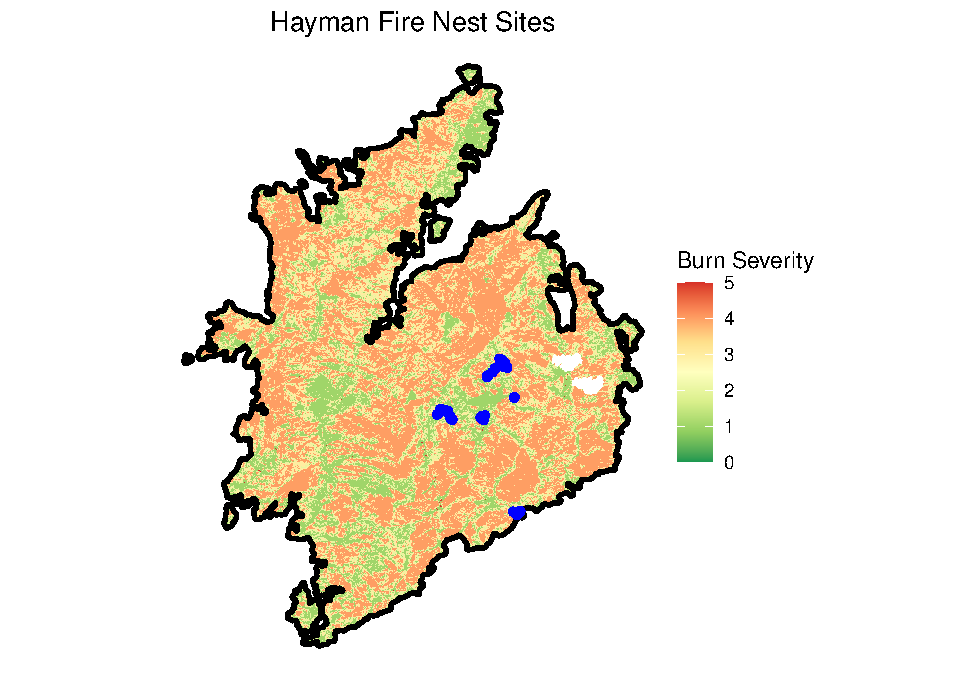
\includegraphics{../manuscript/figures/plot_severity-1.pdf}
\caption{Flammulated Owl nests sampled in the Hayman Fire burn scar
(blue) plotted over Normalized Burn Ratios (NBR) depicting burn
severity.}
\end{figure}

\hypertarget{prey-delivery-rates-by-sex}{%
\section{Prey Delivery Rates by Sex}\label{prey-delivery-rates-by-sex}}

First, we compared average prey delivery rates for males and females at
all study sties at fifteen minute intervals throughout the night.

\hypertarget{read-in-data}{%
\subsubsection{Read in Data}\label{read-in-data}}

Load prey delivery data.

\begin{Shaded}
\begin{Highlighting}[]
\NormalTok{pdOriginal <-}\StringTok{ }\KeywordTok{read.csv}\NormalTok{(}\StringTok{"../data/pd_main.csv"}\NormalTok{)}

\CommentTok{#rename the first column, which imported with a special character}
\KeywordTok{names}\NormalTok{(pdOriginal)[}\DecValTok{1}\NormalTok{] <-}\StringTok{ "nest"}
\end{Highlighting}
\end{Shaded}

Filter to only include M and F (remove `unknown' and `total'), separate
`nest' column into `study\_site' and `territory.'

\begin{Shaded}
\begin{Highlighting}[]
\NormalTok{pdMF <-}\StringTok{ }\NormalTok{pdOriginal }\OperatorTok
\StringTok{  }\KeywordTok{separate}\NormalTok{(}\DataTypeTok{col =}\NormalTok{ nest, }\DataTypeTok{into =} \KeywordTok{c}\NormalTok{(}\StringTok{"study_site"}\NormalTok{, }\StringTok{"territory"}\NormalTok{), }\DataTypeTok{sep =} \DecValTok{1}\NormalTok{, }\DataTypeTok{remove =} \OtherTok{TRUE}\NormalTok{) }\OperatorTok
\StringTok{  }\KeywordTok{filter}\NormalTok{(sex }\OperatorTok{==}\StringTok{ "M"} \OperatorTok{|}\StringTok{ }\NormalTok{sex }\OperatorTok{==}\StringTok{ "F"}\NormalTok{)}
\end{Highlighting}
\end{Shaded}

Check structure of data.

\begin{Shaded}
\begin{Highlighting}[]
\NormalTok{pd_str <-}\StringTok{ }\KeywordTok{str}\NormalTok{(pdMF)}
\end{Highlighting}
\end{Shaded}

\begin{verbatim}
## 'data.frame':    1299 obs. of  55 variables:
##  $ study_site       : chr  "A" "A" "B" "C" ...
##  $ territory        : chr  "29_2007" "29_2007" "7_2005" "S1_1_2005" ...
##  $ year             : int  2007 2007 2005 2005 2005 2005 2006 2006 2014 2004 ...
##  $ obs_date         : Factor w/ 329 levels "","5/30/2006",..: 160 160 35 184 172 69 168 168 163 3 ...
##  $ clutch_size      : Factor w/ 8 levels "","-","?","1",..: 5 5 1 1 1 1 5 5 5 6 ...
##  $ brood_size       : Factor w/ 13 levels "","-","?",">=2",..: 9 9 1 1 1 1 9 9 9 11 ...
##  $ num_fledged      : Factor w/ 11 levels "","-","≥1","≥2",..: 7 7 1 1 1 1 5 5 7 8 ...
##  $ incubation_start : Factor w/ 143 levels "","?","5/13/2012",..: 126 126 1 1 1 1 125 125 112 57 ...
##  $ julian_incubation: int  157 157 NA NA NA NA 157 157 155 151 ...
##  $ nest_age         : Factor w/ 56 levels "","0","1","10",..: 3 3 3 3 3 3 3 3 3 15 ...
##  $ sunset           : int  2021 2021 NA 2025 2023 2020 2023 2023 2026 2019 ...
##  $ sex              : Factor w/ 9 levels "All","F","H",..: 4 2 2 2 2 2 4 2 4 4 ...
##  $ t15              : int  NA NA 0 NA NA NA NA NA 2 NA ...
##  $ t30              : int  NA NA 0 NA NA NA NA NA NA 0 ...
##  $ t45              : int  NA NA 0 NA 0 NA NA NA NA 2 ...
##  $ t60              : int  NA NA 0 NA 0 NA NA NA NA 1 ...
##  $ t75              : int  NA NA 0 NA 0 NA 1 0 NA 3 ...
##  $ t90              : int  NA NA NA 0 0 NA 0 0 NA 0 ...
##  $ t105             : int  NA NA NA 0 0 0 0 0 NA 0 ...
##  $ t120             : int  NA NA NA 0 NA 0 0 0 NA 0 ...
##  $ t135             : int  NA NA NA 0 NA 0 0 0 NA NA ...
##  $ t150             : int  NA NA NA 0 NA 0 1 0 NA NA ...
##  $ t165             : int  NA NA NA NA NA 0 0 0 NA NA ...
##  $ t180             : Factor w/ 12 levels "","0","1","10",..: 3 2 1 1 1 1 1 1 1 1 ...
##  $ t195             : int  3 0 NA NA NA NA NA NA NA NA ...
##  $ t210             : int  2 0 NA NA NA NA NA NA NA NA ...
##  $ t225             : Factor w/ 10 levels "","0","1","11",..: 3 2 1 1 1 1 1 1 1 1 ...
##  $ t240             : int  3 0 NA NA NA NA NA NA NA NA ...
##  $ t255             : int  NA NA NA NA NA NA NA NA NA NA ...
##  $ t270             : int  NA NA NA NA NA NA NA NA NA NA ...
##  $ t285             : int  NA NA NA NA NA NA NA NA NA NA ...
##  $ t300             : int  NA NA NA NA NA NA NA NA NA NA ...
##  $ t315             : int  NA NA NA NA NA NA NA NA NA NA ...
##  $ t330             : int  NA NA NA NA NA NA NA NA NA NA ...
##  $ t345             : int  NA NA NA NA NA NA NA NA NA NA ...
##  $ t360             : int  NA NA NA NA NA NA NA NA NA NA ...
##  $ t375             : int  NA NA NA NA NA NA NA NA NA NA ...
##  $ t390             : int  NA NA NA NA NA NA NA NA NA NA ...
##  $ t405             : int  NA NA NA NA NA NA NA NA NA NA ...
##  $ t420             : int  NA NA NA NA NA NA NA NA NA NA ...
##  $ t435             : int  NA NA NA NA NA NA NA NA NA NA ...
##  $ t450             : int  NA NA NA NA NA NA NA NA NA NA ...
##  $ t465             : int  NA NA NA NA NA NA NA NA NA NA ...
##  $ t480             : int  NA NA NA NA NA NA NA NA NA NA ...
##  $ t495             : int  NA NA NA NA NA NA NA NA NA NA ...
##  $ t510             : int  NA NA NA NA NA NA NA NA NA NA ...
##  $ t525             : int  NA NA NA NA NA NA NA NA NA NA ...
##  $ t540             : int  NA NA NA NA NA NA NA NA NA NA ...
##  $ Comments         : Factor w/ 442 levels "","1 abort","1 abort, capture attempt",..: 388 388 159 117 299 378 59 59 1 408 ...
##  $ obs_time         : Factor w/ 637 levels "","~1950-2205",..: 602 602 37 509 380 510 458 458 268 293 ...
##  $ start_time       : Factor w/ 190 levels "~1950","~2205",..: 165 165 21 110 70 110 93 93 44 46 ...
##  $ stop_time        : Factor w/ 253 levels "?","0:00","1:19",..: 229 229 50 150 72 174 152 152 33 65 ...
##  $ weather          : Factor w/ 387 levels "","\"breezy, 15mph\"",..: 372 372 376 331 350 8 156 156 180 350 ...
##  $ fledge_date      : Factor w/ 144 levels "","?","[predated",..: 1 1 1 1 1 1 1 1 73 34 ...
##  $ fledge_accuracy  : Factor w/ 30 levels "","±0","±1","±2",..: 26 26 25 6 25 6 24 24 2 15 ...
\end{verbatim}

\begin{Shaded}
\begin{Highlighting}[]
\KeywordTok{unique}\NormalTok{(pdMF}\OperatorTok{$}\NormalTok{t180) }\CommentTok{#at least one cell has an asterisk after the value}
\end{Highlighting}
\end{Shaded}

\begin{verbatim}
##  [1] 1  0     4  4* 2  9  10 3  5 
## Levels:  0 1 10 12 2 3 4 4* 5 6 9
\end{verbatim}

\begin{Shaded}
\begin{Highlighting}[]
\KeywordTok{unique}\NormalTok{(pdMF}\OperatorTok{$}\NormalTok{t225) }\CommentTok{#same here}
\end{Highlighting}
\end{Shaded}

\begin{verbatim}
## [1] 1  0     6* 3  2  8  11 7 
## Levels:  0 1 11 2 3 5 6* 7 8
\end{verbatim}

\begin{Shaded}
\begin{Highlighting}[]
\KeywordTok{unique}\NormalTok{(pdMF}\OperatorTok{$}\NormalTok{nest_age) }\CommentTok{#"pred" and "" can be converted to NA}
\end{Highlighting}
\end{Shaded}

\begin{verbatim}
##  [1] 1    2    3    4    5    6    7    8    9    10   11   12   13   14   15  
## [16] 16   17   18   19   20   21   22   23   24   25   26   27   28   29   30  
## [31] 31   32   33   34   35   36   37   38   39   40   41   42   43   44   45  
## [46] 46   47   48   49   50   51   53   100  0    pred     
## 56 Levels:  0 1 10 100 11 12 13 14 15 16 17 18 19 2 20 21 22 23 24 25 26 ... pred
\end{verbatim}

Fix structure by removing asterisks and converting to integer class. NAs
will be generated by coercion, eliminating any blank cells ("``) and
cells containing''pred" (indicating the nest was predated before the
nest age could be confirmed).

\begin{Shaded}
\begin{Highlighting}[]
\CommentTok{#remove asterisks}
\NormalTok{pdClean <-}\StringTok{ }\NormalTok{pdMF }\OperatorTok
\StringTok{  }\KeywordTok{mutate}\NormalTok{(}\DataTypeTok{t180 =} \KeywordTok{gsub}\NormalTok{(}\StringTok{"}\CharTok{\textbackslash{}\textbackslash{}}\StringTok{*"}\NormalTok{, }\StringTok{""}\NormalTok{, t180)) }\OperatorTok
\StringTok{  }\KeywordTok{mutate}\NormalTok{(}\DataTypeTok{t225 =} \KeywordTok{gsub}\NormalTok{(}\StringTok{"}\CharTok{\textbackslash{}\textbackslash{}}\StringTok{*"}\NormalTok{, }\StringTok{""}\NormalTok{, t225)) }


\CommentTok{#change these columns to numeric}
\NormalTok{pdClean}\OperatorTok{$}\NormalTok{t180 <-}\StringTok{ }\KeywordTok{as.integer}\NormalTok{(pdClean}\OperatorTok{$}\NormalTok{t180)}
\NormalTok{pdClean}\OperatorTok{$}\NormalTok{t225 <-}\StringTok{ }\KeywordTok{as.integer}\NormalTok{(pdClean}\OperatorTok{$}\NormalTok{t225)}
\NormalTok{pdClean}\OperatorTok{$}\NormalTok{nest_age <-}\StringTok{ }\KeywordTok{as.integer}\NormalTok{(pdClean}\OperatorTok{$}\NormalTok{nest_age) }
\end{Highlighting}
\end{Shaded}

\hypertarget{organize-data}{%
\subsubsection{Organize Data}\label{organize-data}}

Data was separated by sex (M vs.~F) and by incubation vs.~nestling
stage. Nestling period is defined as nest\_age \textgreater{}= 22 days.
If nest age was not indicated in original dataset, field notes were used
to determine whether nest was in incubation (all eggs) or nestling (at
least one nestling) stage. For these records, the following values were
manually input: nest\_age = 0 for incubation or nest\_age = 100 for
nestling, so that this data could be easily separated from known nest
age. If it was later determined that nest had been predated before
observation, ``pred'' was entered. If the nest stage could not be
determined, it was left blank.``pred'' and "" values were converted to
NA earlier when this column was converted to numeric.

\begin{Shaded}
\begin{Highlighting}[]
\CommentTok{# Create independent dfs for M (nestling and incubation stage) and F (nestling and incubation stage). }

\NormalTok{pdStage_sex <-}\StringTok{ }\NormalTok{pdClean }\OperatorTok
\StringTok{  }\NormalTok{dplyr}\OperatorTok{::}\KeywordTok{select}\NormalTok{(sex, nest_age, t15}\OperatorTok{:}\NormalTok{t240) }\OperatorTok\StringTok{ }\CommentTok{#select relevant columns}
\StringTok{  }\KeywordTok{mutate}\NormalTok{(}
    \DataTypeTok{stage =}
      \KeywordTok{ifelse}\NormalTok{(nest_age }\OperatorTok{<}\StringTok{ }\DecValTok{22}\NormalTok{, }\StringTok{"incubation"}\NormalTok{, }\StringTok{"nestling"}\NormalTok{)) }\OperatorTok\StringTok{ }\CommentTok{#add column for 'stage'}
\StringTok{  }\KeywordTok{drop_na}\NormalTok{(stage) }\CommentTok{#get rid of any rows blank values here, as they can't be used for analysis}
  
\CommentTok{#change column names to remove "t" in front of time interval}
\KeywordTok{colnames}\NormalTok{(pdStage_sex) <-}\StringTok{ }\KeywordTok{c}\NormalTok{(}\StringTok{"sex"}\NormalTok{, }\StringTok{"nest_age"}\NormalTok{, }\StringTok{"15"}\NormalTok{, }\StringTok{"30"}\NormalTok{, }\StringTok{"45"}\NormalTok{, }\StringTok{"60"}\NormalTok{, }\StringTok{"75"}\NormalTok{, }\StringTok{"90"}\NormalTok{, }
                           \StringTok{"105"}\NormalTok{, }\StringTok{"120"}\NormalTok{, }\StringTok{"135"}\NormalTok{, }\StringTok{"150"}\NormalTok{, }\StringTok{"165"}\NormalTok{, }\StringTok{"180"}\NormalTok{, }\StringTok{"195"}\NormalTok{, }\StringTok{"210"}\NormalTok{, }
                           \StringTok{"225"}\NormalTok{, }\StringTok{"240"}\NormalTok{, }\StringTok{"stage"}\NormalTok{)}

\CommentTok{#create independent dfs for each study site and stage}
\NormalTok{pdM_inc <-}\StringTok{ }\NormalTok{pdStage_sex }\OperatorTok
\StringTok{  }\KeywordTok{filter}\NormalTok{(sex }\OperatorTok{==}\StringTok{"M"}\NormalTok{, stage }\OperatorTok{==}\StringTok{ "incubation"}\NormalTok{) }\OperatorTok
\StringTok{  }\NormalTok{dplyr}\OperatorTok{::}\KeywordTok{select}\NormalTok{(}\StringTok{'15'}\OperatorTok{:}\StringTok{'240'}\NormalTok{)}

\NormalTok{pdM_nest <-}\StringTok{ }\NormalTok{pdStage_sex }\OperatorTok\StringTok{ }
\StringTok{  }\KeywordTok{filter}\NormalTok{(sex }\OperatorTok{==}\StringTok{"M"}\NormalTok{, stage }\OperatorTok{==}\StringTok{ "nestling"}\NormalTok{) }\OperatorTok
\StringTok{  }\NormalTok{dplyr}\OperatorTok{::}\KeywordTok{select}\NormalTok{(}\StringTok{'15'}\OperatorTok{:}\StringTok{'240'}\NormalTok{)}

\NormalTok{pdF_inc <-}\StringTok{ }\NormalTok{pdStage_sex }\OperatorTok
\StringTok{  }\KeywordTok{filter}\NormalTok{(sex }\OperatorTok{==}\StringTok{"F"}\NormalTok{, stage }\OperatorTok{==}\StringTok{ "incubation"}\NormalTok{) }\OperatorTok
\StringTok{  }\NormalTok{dplyr}\OperatorTok{::}\KeywordTok{select}\NormalTok{(}\StringTok{'15'}\OperatorTok{:}\StringTok{'240'}\NormalTok{)}
         
\NormalTok{pdF_nest <-}\StringTok{ }\NormalTok{pdStage_sex }\OperatorTok
\StringTok{  }\KeywordTok{filter}\NormalTok{(sex }\OperatorTok{==}\StringTok{"F"}\NormalTok{, stage }\OperatorTok{==}\StringTok{ "nestling"}\NormalTok{) }\OperatorTok
\StringTok{  }\NormalTok{dplyr}\OperatorTok{::}\KeywordTok{select}\NormalTok{(}\StringTok{'15'}\OperatorTok{:}\StringTok{'240'}\NormalTok{)}
\end{Highlighting}
\end{Shaded}

\hypertarget{mean-pd-tables}{%
\subsubsection{Mean PD tables}\label{mean-pd-tables}}

Create four stand-alone data.frames, one for M (incubation), one for M
(nestling), one for F (incubation), and one for F (nestling). These will
be used for t-tests.

\begin{Shaded}
\begin{Highlighting}[]
\NormalTok{meanM_inc <-}\StringTok{ }\KeywordTok{data.frame}\NormalTok{(}
  \DataTypeTok{time =} \KeywordTok{as.numeric}\NormalTok{(}\KeywordTok{colnames}\NormalTok{(pdM_inc)),}
  \DataTypeTok{M_incubation =} \KeywordTok{colMeans}\NormalTok{(pdM_inc, }\DataTypeTok{na.rm =} \OtherTok{TRUE}\NormalTok{))}

\NormalTok{meanM_nest <-}\StringTok{ }\KeywordTok{data.frame}\NormalTok{(}
  \DataTypeTok{time =} \KeywordTok{as.numeric}\NormalTok{(}\KeywordTok{colnames}\NormalTok{(pdM_nest)),}
  \DataTypeTok{M_nestling =} \KeywordTok{colMeans}\NormalTok{(pdM_nest, }\DataTypeTok{na.rm =} \OtherTok{TRUE}\NormalTok{))}

\NormalTok{meanF_inc <-}\StringTok{ }\KeywordTok{data.frame}\NormalTok{(}
  \DataTypeTok{time =} \KeywordTok{as.numeric}\NormalTok{(}\KeywordTok{colnames}\NormalTok{(pdF_inc)),}
  \DataTypeTok{F_incubation =} \KeywordTok{colMeans}\NormalTok{(pdF_inc, }\DataTypeTok{na.rm =} \OtherTok{TRUE}\NormalTok{))}

\NormalTok{meanF_nest <-}\StringTok{ }\KeywordTok{data.frame}\NormalTok{(}
  \DataTypeTok{time =} \KeywordTok{as.numeric}\NormalTok{(}\KeywordTok{colnames}\NormalTok{(pdF_nest)),}
  \DataTypeTok{F_nestling =} \KeywordTok{colMeans}\NormalTok{(pdF_nest, }\DataTypeTok{na.rm =} \OtherTok{TRUE}\NormalTok{))}
\end{Highlighting}
\end{Shaded}

\hypertarget{calculate-confidence-intervals}{%
\subsubsection{Calculate confidence
intervals}\label{calculate-confidence-intervals}}

Apply getCI function across data.frames for each sex and stage.

\begin{Shaded}
\begin{Highlighting}[]
\NormalTok{ciM_inc <-}\StringTok{ }\KeywordTok{apply}\NormalTok{(pdM_inc, }\DecValTok{2}\NormalTok{, }\DataTypeTok{FUN =}\NormalTok{ getCI)}
\NormalTok{ciM_nest <-}\StringTok{ }\KeywordTok{apply}\NormalTok{(pdM_nest, }\DecValTok{2}\NormalTok{, }\DataTypeTok{FUN =}\NormalTok{ getCI)}
\NormalTok{ciF_inc <-}\StringTok{ }\KeywordTok{apply}\NormalTok{(pdF_inc, }\DecValTok{2}\NormalTok{, }\DataTypeTok{FUN =}\NormalTok{ getCI)}
\NormalTok{ciF_nest <-}\StringTok{ }\KeywordTok{apply}\NormalTok{(pdF_nest, }\DecValTok{2}\NormalTok{, }\DataTypeTok{FUN =}\NormalTok{ getCI)}
\end{Highlighting}
\end{Shaded}

Create new data.frames (one for nestling stage and one for incubation
stage) with means and CIs. Remove rows where time \textgreater{} 180 for
ciInc because no data is available for MGSA after this time.

\begin{Shaded}
\begin{Highlighting}[]
\NormalTok{ciInc_sex <-}\StringTok{ }\KeywordTok{data.frame}\NormalTok{(}
    \DataTypeTok{sex =} \KeywordTok{c}\NormalTok{(}\KeywordTok{rep}\NormalTok{(}\StringTok{"M"}\NormalTok{, }\KeywordTok{nrow}\NormalTok{(meanM_inc)), }\KeywordTok{rep}\NormalTok{(}\StringTok{"F"}\NormalTok{, }\KeywordTok{nrow}\NormalTok{(meanF_inc))),}
    \DataTypeTok{mean =} \KeywordTok{c}\NormalTok{(}\KeywordTok{colMeans}\NormalTok{(pdM_inc, }\DataTypeTok{na.rm =} \OtherTok{TRUE}\NormalTok{), }\KeywordTok{colMeans}\NormalTok{(pdF_inc, }\DataTypeTok{na.rm =} \OtherTok{TRUE}\NormalTok{)),}
    \DataTypeTok{ci_l =} \KeywordTok{c}\NormalTok{(ciM_inc[}\DecValTok{1}\NormalTok{,], ciF_inc[}\DecValTok{1}\NormalTok{,]),}
    \DataTypeTok{ci_h =} \KeywordTok{c}\NormalTok{(ciM_inc[}\DecValTok{2}\NormalTok{,], ciF_inc[}\DecValTok{2}\NormalTok{,]),}
    \DataTypeTok{time =} \KeywordTok{c}\NormalTok{(}\KeywordTok{as.numeric}\NormalTok{(}\KeywordTok{rownames}\NormalTok{(meanM_inc)), }\KeywordTok{as.numeric}\NormalTok{(}\KeywordTok{rownames}\NormalTok{(meanF_inc))),}
    \DataTypeTok{stage =} \StringTok{"Incubation"}\NormalTok{)}


\NormalTok{ciNest_sex <-}\StringTok{ }\KeywordTok{data.frame}\NormalTok{(}
    \DataTypeTok{sex =} \KeywordTok{c}\NormalTok{(}\KeywordTok{rep}\NormalTok{(}\StringTok{"M"}\NormalTok{, }\KeywordTok{nrow}\NormalTok{(meanM_nest)), }\KeywordTok{rep}\NormalTok{(}\StringTok{"F"}\NormalTok{, }\KeywordTok{nrow}\NormalTok{(meanF_nest))),}
    \DataTypeTok{mean =} \KeywordTok{c}\NormalTok{(}\KeywordTok{colMeans}\NormalTok{(pdM_nest, }\DataTypeTok{na.rm =} \OtherTok{TRUE}\NormalTok{), }\KeywordTok{colMeans}\NormalTok{(pdF_nest, }\DataTypeTok{na.rm =} \OtherTok{TRUE}\NormalTok{)),}
    \DataTypeTok{ci_l =} \KeywordTok{c}\NormalTok{(ciM_nest[}\DecValTok{1}\NormalTok{,], ciF_nest[}\DecValTok{1}\NormalTok{,]),}
    \DataTypeTok{ci_h =} \KeywordTok{c}\NormalTok{(ciM_nest[}\DecValTok{2}\NormalTok{,], ciF_nest[}\DecValTok{2}\NormalTok{,]),}
    \DataTypeTok{time =} \KeywordTok{c}\NormalTok{(}\KeywordTok{as.numeric}\NormalTok{(}\KeywordTok{rownames}\NormalTok{(meanM_nest)), }\KeywordTok{as.numeric}\NormalTok{(}\KeywordTok{rownames}\NormalTok{(meanF_nest))),}
    \DataTypeTok{stage =} \StringTok{"Nestling"}\NormalTok{)}
\end{Highlighting}
\end{Shaded}

\hypertarget{test-for-difference}{%
\subsubsection{Test for Difference}\label{test-for-difference}}

Test for normality for each time interval in M\_inc, M\_nest, and
F\_nest (excluded pdF\_inc because all values = 0, as female did not
deliver prey while incubating).

\begin{Shaded}
\begin{Highlighting}[]
\CommentTok{# Store results of testNormality in new df}
\NormalTok{normality_sex <-}\StringTok{ }\KeywordTok{data.frame}\NormalTok{(}
  \DataTypeTok{M_inc =} \KeywordTok{testNormality}\NormalTok{(pdM_inc, }\DecValTok{2}\NormalTok{), }
  \DataTypeTok{M_nest =} \KeywordTok{testNormality}\NormalTok{(pdM_nest, }\DecValTok{2}\NormalTok{), }
  \DataTypeTok{F_nest =} \KeywordTok{testNormality}\NormalTok{(pdF_nest, }\DecValTok{2}\NormalTok{)}
\NormalTok{  )}

\CommentTok{# Test if any values are not significant}
\KeywordTok{any}\NormalTok{(normality_sex }\OperatorTok{>=}\StringTok{ }\FloatTok{0.05}\NormalTok{)}
\end{Highlighting}
\end{Shaded}

\begin{verbatim}
## [1] FALSE
\end{verbatim}

All vectors in each list are significantly different from null
hypothesis of Shapiro-Wilk normality test, meaning that no vector is
normally distributed. Therefore, we use the unpaired two-sample Wilcoxon
test to compare median values of M and F prey deliveries during each
time interval, for incubation and nestling stages.

\begin{Shaded}
\begin{Highlighting}[]
\CommentTok{# Incubation Stage}
\NormalTok{wilcox_inc_sex <-}\StringTok{ }\KeywordTok{testWilcox}\NormalTok{(pdM_inc, pdF_inc)}
\KeywordTok{print}\NormalTok{(wilcox_inc_sex)}
\end{Highlighting}
\end{Shaded}

\begin{verbatim}
##          values ind
## 1  1.019974e-06  15
## 2  1.842053e-13  30
## 3  8.812928e-17  45
## 4  4.876663e-23  60
## 5  4.979458e-17  75
## 6  1.416015e-11  90
## 7  2.042524e-11 105
## 8  1.146429e-08 120
## 9  6.929846e-06 135
## 10 1.262014e-04 150
## 11 8.600343e-04 165
## 12 5.766232e-05 180
## 13 4.327965e-03 195
## 14 1.005653e-02 210
## 15 1.204784e-01 225
## 16 3.815739e-01 240
\end{verbatim}

\begin{Shaded}
\begin{Highlighting}[]
\KeywordTok{any}\NormalTok{(wilcox_inc_sex}\OperatorTok{$}\NormalTok{values }\OperatorTok{<=}\StringTok{ }\FloatTok{0.05}\NormalTok{) }\CommentTok{#test if any p.values are sig diff}
\end{Highlighting}
\end{Shaded}

\begin{verbatim}
## [1] TRUE
\end{verbatim}

\begin{Shaded}
\begin{Highlighting}[]
\KeywordTok{all}\NormalTok{(wilcox_inc_sex}\OperatorTok{$}\NormalTok{values }\OperatorTok{<=}\StringTok{ }\FloatTok{0.05}\NormalTok{) }\CommentTok{#test if all p.values are sig diff}
\end{Highlighting}
\end{Shaded}

\begin{verbatim}
## [1] FALSE
\end{verbatim}

\begin{Shaded}
\begin{Highlighting}[]
\NormalTok{dplyr}\OperatorTok{::}\KeywordTok{filter}\NormalTok{(wilcox_inc_sex, values }\OperatorTok{<=}\StringTok{ }\FloatTok{0.05}\NormalTok{) }\CommentTok{#print which rows have sig diff p.value }
\end{Highlighting}
\end{Shaded}

\begin{verbatim}
##          values ind
## 1  1.019974e-06  15
## 2  1.842053e-13  30
## 3  8.812928e-17  45
## 4  4.876663e-23  60
## 5  4.979458e-17  75
## 6  1.416015e-11  90
## 7  2.042524e-11 105
## 8  1.146429e-08 120
## 9  6.929846e-06 135
## 10 1.262014e-04 150
## 11 8.600343e-04 165
## 12 5.766232e-05 180
## 13 4.327965e-03 195
## 14 1.005653e-02 210
\end{verbatim}

\begin{Shaded}
\begin{Highlighting}[]
\CommentTok{# Nestling Stage}
\NormalTok{wilcox_nest_sex <-}\StringTok{ }\KeywordTok{testWilcox}\NormalTok{(pdM_nest, pdF_nest)}
\KeywordTok{print}\NormalTok{(wilcox_nest_sex)}
\end{Highlighting}
\end{Shaded}

\begin{verbatim}
##          values ind
## 1  6.653744e-05  15
## 2  5.385296e-11  30
## 3  8.915504e-08  45
## 4  6.881521e-07  60
## 5  1.758982e-13  75
## 6  2.404649e-10  90
## 7  3.977980e-06 105
## 8  2.672459e-06 120
## 9  9.038698e-09 135
## 10 1.039497e-04 150
## 11 2.751843e-05 165
## 12 3.539645e-06 180
## 13 2.332547e-02 195
## 14 2.006606e-04 210
## 15 2.127009e-04 225
## 16 2.171260e-04 240
\end{verbatim}

\begin{Shaded}
\begin{Highlighting}[]
\KeywordTok{any}\NormalTok{(wilcox_nest_sex}\OperatorTok{$}\NormalTok{values }\OperatorTok{<=}\StringTok{ }\FloatTok{0.05}\NormalTok{) }\CommentTok{#test if any p.values are sig diff}
\end{Highlighting}
\end{Shaded}

\begin{verbatim}
## [1] TRUE
\end{verbatim}

\begin{Shaded}
\begin{Highlighting}[]
\KeywordTok{all}\NormalTok{(wilcox_nest_sex}\OperatorTok{$}\NormalTok{values }\OperatorTok{<=}\StringTok{ }\FloatTok{0.05}\NormalTok{) }\CommentTok{#test if all p.values are sig diff}
\end{Highlighting}
\end{Shaded}

\begin{verbatim}
## [1] TRUE
\end{verbatim}

From the Wilcoxon tests, we see that all median time intervals during
the nestling stage are significantly different between males and
females. However, during the incubation stage, median prey delivery
rates at time = 2255 and time = 240 are not significantly different
between males and females.

\hypertarget{plot}{%
\subsubsection{Plot}\label{plot}}

Incubation (including star indicating non-significant Wilcoxon test at t
= 225 and t = 240):

\begin{Shaded}
\begin{Highlighting}[]
\NormalTok{plotInc_sex <-}\StringTok{ }\KeywordTok{ggplot}\NormalTok{(}\DataTypeTok{data =}\NormalTok{ ciInc_sex) }\OperatorTok{+}
\StringTok{  }\KeywordTok{geom_point}\NormalTok{(}\KeywordTok{aes}\NormalTok{(}\DataTypeTok{x =}\NormalTok{ time, }\DataTypeTok{y =}\NormalTok{ mean, }\DataTypeTok{color =}\NormalTok{ sex, }\DataTypeTok{group =}\NormalTok{ sex),}
             \DataTypeTok{position =} \KeywordTok{position_dodge}\NormalTok{(}\DataTypeTok{width=}\FloatTok{0.75}\NormalTok{)) }\OperatorTok{+}
\StringTok{  }\KeywordTok{geom_errorbar}\NormalTok{(}\KeywordTok{aes}\NormalTok{(}\DataTypeTok{x=}\NormalTok{time, }\DataTypeTok{ymax =}\NormalTok{ ci_h, }\DataTypeTok{ymin=}\NormalTok{ci_l, }\DataTypeTok{color =}\NormalTok{ sex, }
                    \DataTypeTok{group =}\NormalTok{ sex),}
                \DataTypeTok{position =} \KeywordTok{position_dodge}\NormalTok{(}\DataTypeTok{width=}\FloatTok{0.75}\NormalTok{)) }\OperatorTok{+}
\StringTok{  }\KeywordTok{labs}\NormalTok{(}\DataTypeTok{x =} \StringTok{"Time After Sunset (minutes)"}\NormalTok{, }\DataTypeTok{y =} \StringTok{"Mean Prey Deliveries"}\NormalTok{, }
       \DataTypeTok{title =} \StringTok{"Incubation"}\NormalTok{, }\DataTypeTok{color =} \StringTok{"Sex"}\NormalTok{) }\OperatorTok{+}
\StringTok{  }\KeywordTok{theme_minimal}\NormalTok{() }\OperatorTok{+}
\StringTok{  }\KeywordTok{theme}\NormalTok{(}\DataTypeTok{plot.title =} \KeywordTok{element_text}\NormalTok{(}\DataTypeTok{hjust =} \FloatTok{0.5}\NormalTok{)) }\OperatorTok{+}
\StringTok{  }\KeywordTok{geom_point}\NormalTok{(}\KeywordTok{aes}\NormalTok{(}\DataTypeTok{x =} \DecValTok{225}\NormalTok{, }\DataTypeTok{y =} \FloatTok{3.0}\NormalTok{), }\DataTypeTok{shape =} \DecValTok{8}\NormalTok{, }\DataTypeTok{stroke =} \FloatTok{0.1}\NormalTok{) }\OperatorTok{+}
\StringTok{  }\KeywordTok{geom_point}\NormalTok{(}\KeywordTok{aes}\NormalTok{(}\DataTypeTok{x =} \DecValTok{240}\NormalTok{, }\DataTypeTok{y =} \FloatTok{2.5}\NormalTok{), }\DataTypeTok{shape =} \DecValTok{8}\NormalTok{, }\DataTypeTok{stroke =} \FloatTok{0.1}\NormalTok{)}
\end{Highlighting}
\end{Shaded}

Nestling:

\begin{Shaded}
\begin{Highlighting}[]
\NormalTok{plotNest_sex <-}\StringTok{ }\KeywordTok{ggplot}\NormalTok{(}\DataTypeTok{data =}\NormalTok{ ciNest_sex) }\OperatorTok{+}
\StringTok{  }\KeywordTok{geom_point}\NormalTok{(}\KeywordTok{aes}\NormalTok{(}\DataTypeTok{x =}\NormalTok{ time, }\DataTypeTok{y =}\NormalTok{ mean, }\DataTypeTok{color =}\NormalTok{ sex, }\DataTypeTok{group =}\NormalTok{ sex),}
             \DataTypeTok{position =} \KeywordTok{position_dodge}\NormalTok{(}\DataTypeTok{width=}\FloatTok{0.75}\NormalTok{)) }\OperatorTok{+}
\StringTok{  }\KeywordTok{geom_errorbar}\NormalTok{(}\KeywordTok{aes}\NormalTok{(}\DataTypeTok{x=}\NormalTok{time, }\DataTypeTok{ymax =}\NormalTok{ ci_h, }\DataTypeTok{ymin=}\NormalTok{ci_l, }\DataTypeTok{color =}\NormalTok{ sex, }
                    \DataTypeTok{group =}\NormalTok{ sex),}
                \DataTypeTok{position =} \KeywordTok{position_dodge}\NormalTok{(}\DataTypeTok{width=}\FloatTok{0.75}\NormalTok{)) }\OperatorTok{+}
\StringTok{  }\KeywordTok{labs}\NormalTok{(}\DataTypeTok{x =} \StringTok{"Time After Sunset (minutes)"}\NormalTok{, }\DataTypeTok{y =} \StringTok{"Mean Prey Deliveries"}\NormalTok{, }
       \DataTypeTok{title =} \StringTok{"Nestling"}\NormalTok{, }\DataTypeTok{color =} \StringTok{"Sex"}\NormalTok{) }\OperatorTok{+}
\StringTok{  }\KeywordTok{theme_minimal}\NormalTok{() }\OperatorTok{+}
\StringTok{  }\KeywordTok{theme}\NormalTok{(}\DataTypeTok{plot.title =} \KeywordTok{element_text}\NormalTok{(}\DataTypeTok{hjust =} \FloatTok{0.5}\NormalTok{)) }
\end{Highlighting}
\end{Shaded}

The final plot compares both incubation and nestling stages.

\begin{Shaded}
\begin{Highlighting}[]
\KeywordTok{grid.arrange}\NormalTok{(plotInc_sex, plotNest_sex)}
\end{Highlighting}
\end{Shaded}

\begin{figure}
\centering
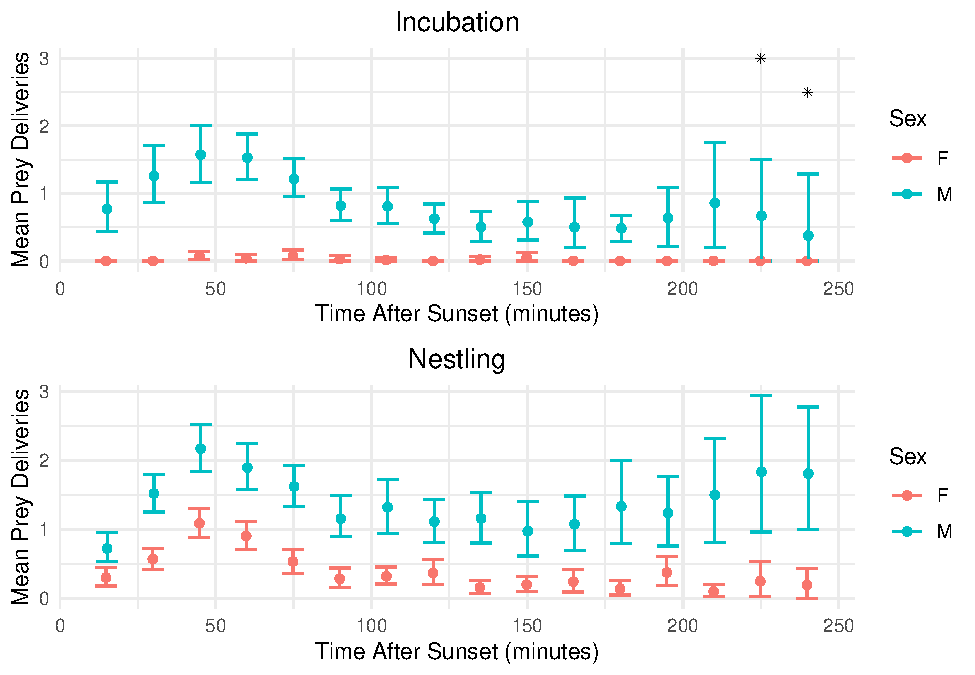
\includegraphics{../manuscript/figures/plot_sex-1.pdf}
\caption{Mean prey deliveries during the incubation stage (top) and
nestling stage (bottom). Males are shown in bue and females in red.
Stars indicate non-significant differences in medians based on unpaired
two-sample Wilcoxon tests.}
\end{figure}

\hypertarget{prey-delivery-rates-by-site}{%
\section{Prey Delivery Rates by
Site}\label{prey-delivery-rates-by-site}}

The original spreadsheet contains prey delivery data from two other
studies that were not considered in this analysis. Therefore, they were
filtered out, and ``B'' (MGSA) and ``C'' (HFSA) were preserved for the
analysis. Females were also excluded because here was not sufficient
data for reliable analysis.

\begin{Shaded}
\begin{Highlighting}[]
\NormalTok{pdHM <-}\StringTok{ }\NormalTok{pdClean }\OperatorTok
\StringTok{  }\KeywordTok{filter}\NormalTok{(study_site }\OperatorTok{==}\StringTok{ "B"} \OperatorTok{|}\StringTok{ }\NormalTok{study_site }\OperatorTok{==}\StringTok{ "C"}\NormalTok{, sex }\OperatorTok{==}\StringTok{ "M"}\NormalTok{)}
\end{Highlighting}
\end{Shaded}

\hypertarget{organize-data-1}{%
\subsubsection{Organize Data}\label{organize-data-1}}

Data was separated by study site (HFSA vs.~MGSA) and by incubation
vs.~nestling stage. Since the last observation for HFSA is at time =
240, we'll end the first data.frame there.

Then, create data.frames for each study site and stage. End incubation
data.frames at t = 180 and nestling data.frames at t = 240 because this
is the maximum time when there is data for both sites.

\begin{Shaded}
\begin{Highlighting}[]
\CommentTok{#create independet dfs for HFSA (nestling and incubation stage) and MGSA (nestling and incubation state). }

\CommentTok{#select relevant columns, add column for stage, rename study sites, drop NAs}
\NormalTok{pdStage_site <-}\StringTok{ }\NormalTok{pdClean }\OperatorTok
\StringTok{  }\NormalTok{dplyr}\OperatorTok{::}\KeywordTok{select}\NormalTok{(study_site, nest_age, t15}\OperatorTok{:}\NormalTok{t240) }\OperatorTok
\StringTok{  }\KeywordTok{mutate}\NormalTok{(}
    \DataTypeTok{stage =}
      \KeywordTok{ifelse}\NormalTok{(nest_age }\OperatorTok{<}\StringTok{ }\DecValTok{22}\NormalTok{, }\StringTok{"incubation"}\NormalTok{, }\StringTok{"nestling"}\NormalTok{),}
    \DataTypeTok{study_site =}
      \KeywordTok{ifelse}\NormalTok{(study_site }\OperatorTok{==}\StringTok{ "B"}\NormalTok{, }\StringTok{"MGSA"}\NormalTok{, }\StringTok{"HFSA"}\NormalTok{)) }\OperatorTok
\StringTok{  }\KeywordTok{drop_na}\NormalTok{(stage)}

\CommentTok{#change column names to remove "t" in front of time interval}
\KeywordTok{colnames}\NormalTok{(pdStage_site) <-}\StringTok{ }\KeywordTok{c}\NormalTok{(}\StringTok{"study_site"}\NormalTok{, }\StringTok{"nest_age"}\NormalTok{, }\StringTok{"15"}\NormalTok{, }\StringTok{"30"}\NormalTok{, }\StringTok{"45"}\NormalTok{, }\StringTok{"60"}\NormalTok{, }
                            \StringTok{"75"}\NormalTok{, }\StringTok{"90"}\NormalTok{, }\StringTok{"105"}\NormalTok{, }\StringTok{"120"}\NormalTok{, }\StringTok{"135"}\NormalTok{, }\StringTok{"150"}\NormalTok{, }\StringTok{"165"}\NormalTok{, }\StringTok{"180"}\NormalTok{, }
                            \StringTok{"195"}\NormalTok{, }\StringTok{"210"}\NormalTok{, }\StringTok{"225"}\NormalTok{, }\StringTok{"240"}\NormalTok{, }\StringTok{"stage"}\NormalTok{)}

\CommentTok{#create independent dfs for each study site and stage}
\NormalTok{pdHFSA_inc <-}\StringTok{ }\NormalTok{pdStage_site }\OperatorTok
\StringTok{  }\KeywordTok{filter}\NormalTok{(study_site }\OperatorTok{==}\StringTok{"HFSA"}\NormalTok{, stage }\OperatorTok{==}\StringTok{ "incubation"}\NormalTok{) }\OperatorTok
\StringTok{  }\NormalTok{dplyr}\OperatorTok{::}\KeywordTok{select}\NormalTok{(}\StringTok{'15'}\OperatorTok{:}\StringTok{'180'}\NormalTok{)}

\NormalTok{pdHFSA_nest <-}\StringTok{ }\NormalTok{pdStage_site }\OperatorTok\StringTok{ }
\StringTok{  }\KeywordTok{filter}\NormalTok{(study_site }\OperatorTok{==}\StringTok{"HFSA"}\NormalTok{, stage }\OperatorTok{==}\StringTok{ "nestling"}\NormalTok{) }\OperatorTok
\StringTok{  }\NormalTok{dplyr}\OperatorTok{::}\KeywordTok{select}\NormalTok{(}\StringTok{'15'}\OperatorTok{:}\StringTok{'240'}\NormalTok{)}

\NormalTok{pdMGSA_inc <-}\StringTok{ }\NormalTok{pdStage_site }\OperatorTok
\StringTok{  }\KeywordTok{filter}\NormalTok{(study_site }\OperatorTok{==}\StringTok{"MGSA"}\NormalTok{, stage }\OperatorTok{==}\StringTok{ "incubation"}\NormalTok{) }\OperatorTok
\StringTok{  }\NormalTok{dplyr}\OperatorTok{::}\KeywordTok{select}\NormalTok{(}\StringTok{'15'}\OperatorTok{:}\StringTok{'180'}\NormalTok{)}
         
\NormalTok{pdMGSA_nest <-}\StringTok{ }\NormalTok{pdStage_site }\OperatorTok
\StringTok{  }\KeywordTok{filter}\NormalTok{(study_site }\OperatorTok{==}\StringTok{"MGSA"}\NormalTok{, stage }\OperatorTok{==}\StringTok{ "nestling"}\NormalTok{) }\OperatorTok
\StringTok{  }\NormalTok{dplyr}\OperatorTok{::}\KeywordTok{select}\NormalTok{(}\StringTok{'15'}\OperatorTok{:}\StringTok{'240'}\NormalTok{)}
\end{Highlighting}
\end{Shaded}

\hypertarget{mean-pd-tables-1}{%
\subsubsection{Mean PD tables}\label{mean-pd-tables-1}}

Create four stand-alone data.frames, one for HFSA (incubation), one for
HFSA (nestling), one for MGSA (incubation), and one for MGSA (nestling).

\begin{Shaded}
\begin{Highlighting}[]
\NormalTok{meanHFSA_inc <-}\StringTok{ }\KeywordTok{data.frame}\NormalTok{(}
  \DataTypeTok{time =} \KeywordTok{as.numeric}\NormalTok{(}\KeywordTok{colnames}\NormalTok{(pdHFSA_inc)),}
  \DataTypeTok{HFSA_incubation =} \KeywordTok{colMeans}\NormalTok{(pdHFSA_inc, }\DataTypeTok{na.rm =} \OtherTok{TRUE}\NormalTok{))}

\NormalTok{meanHFSA_nest <-}\StringTok{ }\KeywordTok{data.frame}\NormalTok{(}
  \DataTypeTok{time =} \KeywordTok{as.numeric}\NormalTok{(}\KeywordTok{colnames}\NormalTok{(pdHFSA_nest)),}
  \DataTypeTok{HFSA_nestling =} \KeywordTok{colMeans}\NormalTok{(pdHFSA_nest, }\DataTypeTok{na.rm =} \OtherTok{TRUE}\NormalTok{))}

\NormalTok{meanMGSA_inc <-}\StringTok{ }\KeywordTok{data.frame}\NormalTok{(}
  \DataTypeTok{time =} \KeywordTok{as.numeric}\NormalTok{(}\KeywordTok{colnames}\NormalTok{(pdMGSA_inc)),}
  \DataTypeTok{MGSA_incubation =} \KeywordTok{colMeans}\NormalTok{(pdMGSA_inc, }\DataTypeTok{na.rm =} \OtherTok{TRUE}\NormalTok{))}

\NormalTok{meanMGSA_nest <-}\StringTok{ }\KeywordTok{data.frame}\NormalTok{(}
  \DataTypeTok{time =} \KeywordTok{as.numeric}\NormalTok{(}\KeywordTok{colnames}\NormalTok{(pdMGSA_nest)),}
  \DataTypeTok{MGSA_nestling =} \KeywordTok{colMeans}\NormalTok{(pdMGSA_nest, }\DataTypeTok{na.rm =} \OtherTok{TRUE}\NormalTok{))}
\end{Highlighting}
\end{Shaded}

\hypertarget{calculate-confidence-intervals-1}{%
\subsubsection{Calculate confidence
intervals}\label{calculate-confidence-intervals-1}}

Apply getCI across each data.frame, taking each time interval as vector.

\begin{Shaded}
\begin{Highlighting}[]
\NormalTok{ciHFSA_inc <-}\StringTok{ }\KeywordTok{apply}\NormalTok{(pdHFSA_inc, }\DecValTok{2}\NormalTok{, }\DataTypeTok{FUN =}\NormalTok{ getCI)}
\NormalTok{ciHFSA_nest <-}\StringTok{ }\KeywordTok{apply}\NormalTok{(pdHFSA_nest, }\DecValTok{2}\NormalTok{, }\DataTypeTok{FUN =}\NormalTok{ getCI)}
\NormalTok{ciMGSA_inc <-}\StringTok{ }\KeywordTok{apply}\NormalTok{(pdMGSA_inc, }\DecValTok{2}\NormalTok{, }\DataTypeTok{FUN =}\NormalTok{ getCI)}
\NormalTok{ciMGSA_nest <-}\StringTok{ }\KeywordTok{apply}\NormalTok{(pdMGSA_nest, }\DecValTok{2}\NormalTok{, }\DataTypeTok{FUN =}\NormalTok{ getCI)}
\end{Highlighting}
\end{Shaded}

Add CIs to a data.frame.

\begin{Shaded}
\begin{Highlighting}[]
\NormalTok{ciInc <-}\StringTok{ }\KeywordTok{data.frame}\NormalTok{(}
    \DataTypeTok{study_area =} \KeywordTok{c}\NormalTok{(}\KeywordTok{rep}\NormalTok{(}\StringTok{"HFSA"}\NormalTok{, }\KeywordTok{nrow}\NormalTok{(meanHFSA_inc)), }\KeywordTok{rep}\NormalTok{(}\StringTok{"MGSA"}\NormalTok{, }\KeywordTok{nrow}\NormalTok{(meanMGSA_inc))),}
    \DataTypeTok{mean =} \KeywordTok{c}\NormalTok{(}\KeywordTok{colMeans}\NormalTok{(pdHFSA_inc, }\DataTypeTok{na.rm =} \OtherTok{TRUE}\NormalTok{), }\KeywordTok{colMeans}\NormalTok{(pdMGSA_inc, }\DataTypeTok{na.rm =} \OtherTok{TRUE}\NormalTok{)),}
    \DataTypeTok{ci_l =} \KeywordTok{c}\NormalTok{(ciHFSA_inc[}\DecValTok{1}\NormalTok{,], ciMGSA_inc[}\DecValTok{1}\NormalTok{,]),}
    \DataTypeTok{ci_h =} \KeywordTok{c}\NormalTok{(ciHFSA_inc[}\DecValTok{2}\NormalTok{,], ciMGSA_inc[}\DecValTok{2}\NormalTok{,]),}
    \DataTypeTok{time =} \KeywordTok{c}\NormalTok{(}\KeywordTok{as.numeric}\NormalTok{(}\KeywordTok{rownames}\NormalTok{(meanHFSA_inc)), }\KeywordTok{as.numeric}\NormalTok{(}\KeywordTok{rownames}\NormalTok{(meanMGSA_inc))),}
    \DataTypeTok{stage =} \StringTok{"Incubation"}\NormalTok{)}


\NormalTok{ciNest <-}\StringTok{ }\KeywordTok{data.frame}\NormalTok{(}
    \DataTypeTok{study_area =} \KeywordTok{c}\NormalTok{(}\KeywordTok{rep}\NormalTok{(}\StringTok{"HFSA"}\NormalTok{, }\KeywordTok{nrow}\NormalTok{(meanHFSA_nest)), }\KeywordTok{rep}\NormalTok{(}\StringTok{"MGSA"}\NormalTok{, }\KeywordTok{nrow}\NormalTok{(meanMGSA_nest))),}
    \DataTypeTok{mean =} \KeywordTok{c}\NormalTok{(}\KeywordTok{colMeans}\NormalTok{(pdHFSA_nest, }\DataTypeTok{na.rm =} \OtherTok{TRUE}\NormalTok{), }\KeywordTok{colMeans}\NormalTok{(pdMGSA_nest, }\DataTypeTok{na.rm =} \OtherTok{TRUE}\NormalTok{)),}
    \DataTypeTok{ci_l =} \KeywordTok{c}\NormalTok{(ciHFSA_nest[}\DecValTok{1}\NormalTok{,], ciMGSA_nest[}\DecValTok{1}\NormalTok{,]),}
    \DataTypeTok{ci_h =} \KeywordTok{c}\NormalTok{(ciHFSA_nest[}\DecValTok{2}\NormalTok{,], ciMGSA_nest[}\DecValTok{2}\NormalTok{,]),}
    \DataTypeTok{time =} \KeywordTok{c}\NormalTok{(}\KeywordTok{as.numeric}\NormalTok{(}\KeywordTok{rownames}\NormalTok{(meanHFSA_nest)), }\KeywordTok{as.numeric}\NormalTok{(}\KeywordTok{rownames}\NormalTok{(meanMGSA_nest))),}
    \DataTypeTok{stage =} \StringTok{"Nestling"}\NormalTok{)}
\end{Highlighting}
\end{Shaded}

\hypertarget{test-for-difference-1}{%
\subsubsection{Test for Difference}\label{test-for-difference-1}}

Test for normality for each time interval in pdMGSA\_inc, pdMGSA\_nest,
pdHFSA\_inc, and pdHFSA\_nest.

\begin{Shaded}
\begin{Highlighting}[]
\CommentTok{# Store results of testNormality in new df}
\NormalTok{normality_site <-}\StringTok{ }\KeywordTok{list}\NormalTok{(}
  \DataTypeTok{MGSA_inc =} \KeywordTok{testNormality}\NormalTok{(pdMGSA_inc, }\DecValTok{2}\NormalTok{), }
  \DataTypeTok{MGSA_nest =} \KeywordTok{testNormality}\NormalTok{(pdMGSA_nest, }\DecValTok{2}\NormalTok{), }
  \DataTypeTok{HFSA_inc =} \KeywordTok{testNormality}\NormalTok{(pdHFSA_inc, }\DecValTok{2}\NormalTok{),}
  \DataTypeTok{HFSA_nest =} \KeywordTok{testNormality}\NormalTok{(pdHFSA_nest, }\DecValTok{2}\NormalTok{))}

\CommentTok{# Test if any values are not significant}
\KeywordTok{sapply}\NormalTok{(normality_site, }\DataTypeTok{FUN =} \ControlFlowTok{function}\NormalTok{(x)\{}\KeywordTok{any}\NormalTok{(x }\OperatorTok{>=}\StringTok{ }\FloatTok{0.05}\NormalTok{)\})}
\end{Highlighting}
\end{Shaded}

\begin{verbatim}
##  MGSA_inc MGSA_nest  HFSA_inc HFSA_nest 
##     FALSE     FALSE     FALSE     FALSE
\end{verbatim}

All vectors in each list are significantly different from null
hypothesis of Shapiro-Wilk normality test, meaning that no vector is
normally distributed. Therefore, we use the unpaired two-sample Wilcoxon
test to compare median values for each time interval in MGSA and HFSA,
for incubation and nestling stages.

\begin{Shaded}
\begin{Highlighting}[]
\CommentTok{# Incubation Stage}
\NormalTok{wilcox_inc_site <-}\StringTok{ }\KeywordTok{testWilcox}\NormalTok{(pdMGSA_inc, pdHFSA_inc)}
\KeywordTok{print}\NormalTok{(wilcox_inc_site)}
\end{Highlighting}
\end{Shaded}

\begin{verbatim}
##       values ind
## 1  0.9242557  15
## 2  0.8559074  30
## 3  0.0509752  45
## 4  0.3946968  60
## 5  0.2241870  75
## 6  0.2673633  90
## 7  0.6397543 105
## 8  0.9371807 120
## 9  0.8637855 135
## 10 0.1421301 150
## 11 0.3553358 165
## 12 0.8206028 180
\end{verbatim}

\begin{Shaded}
\begin{Highlighting}[]
\KeywordTok{any}\NormalTok{(wilcox_inc_site}\OperatorTok{$}\NormalTok{values }\OperatorTok{<=}\StringTok{ }\FloatTok{0.05}\NormalTok{) }\CommentTok{#test if any p.values are sig dif}
\end{Highlighting}
\end{Shaded}

\begin{verbatim}
## [1] FALSE
\end{verbatim}

\begin{Shaded}
\begin{Highlighting}[]
\KeywordTok{all}\NormalTok{(wilcox_inc_site}\OperatorTok{$}\NormalTok{values }\OperatorTok{>}\StringTok{ }\FloatTok{0.05}\NormalTok{) }\CommentTok{#test if all p.values are not significant }
\end{Highlighting}
\end{Shaded}

\begin{verbatim}
## [1] TRUE
\end{verbatim}

\begin{Shaded}
\begin{Highlighting}[]
\CommentTok{# Nestling Stage}
\NormalTok{wilcox_nest_site <-}\StringTok{ }\KeywordTok{testWilcox}\NormalTok{(pdMGSA_nest, pdHFSA_nest)}
\KeywordTok{print}\NormalTok{(wilcox_inc_site)}
\end{Highlighting}
\end{Shaded}

\begin{verbatim}
##       values ind
## 1  0.9242557  15
## 2  0.8559074  30
## 3  0.0509752  45
## 4  0.3946968  60
## 5  0.2241870  75
## 6  0.2673633  90
## 7  0.6397543 105
## 8  0.9371807 120
## 9  0.8637855 135
## 10 0.1421301 150
## 11 0.3553358 165
## 12 0.8206028 180
\end{verbatim}

\begin{Shaded}
\begin{Highlighting}[]
\KeywordTok{any}\NormalTok{(wilcox_nest_site}\OperatorTok{$}\NormalTok{values }\OperatorTok{<=}\StringTok{ }\FloatTok{0.05}\NormalTok{) }\CommentTok{#test if any p.values are sig diff}
\end{Highlighting}
\end{Shaded}

\begin{verbatim}
## [1] TRUE
\end{verbatim}

\begin{Shaded}
\begin{Highlighting}[]
\NormalTok{dplyr}\OperatorTok{::}\KeywordTok{filter}\NormalTok{(wilcox_nest_site, values }\OperatorTok{<=}\StringTok{ }\FloatTok{0.05}\NormalTok{) }\CommentTok{#print which row has sig diff p.value}
\end{Highlighting}
\end{Shaded}

\begin{verbatim}
##       values ind
## 1 0.04904887 165
\end{verbatim}

From the Wilcoxon tests, we see that no median time intervals during the
incubation stage are different between MGSA and HFSA. However, during
the nestling stage, median prey delivery rates at time = 165 are
significantly different between MGSA and HFSA.

\hypertarget{plot-1}{%
\subsubsection{Plot}\label{plot-1}}

Mean prey deliveries throughout night in incubation stage:

\begin{Shaded}
\begin{Highlighting}[]
\NormalTok{plotInc_site <-}\StringTok{ }\KeywordTok{ggplot}\NormalTok{(}\DataTypeTok{data =}\NormalTok{ ciInc) }\OperatorTok{+}
\StringTok{  }\KeywordTok{geom_point}\NormalTok{(}\KeywordTok{aes}\NormalTok{(}\DataTypeTok{x =}\NormalTok{ time, }\DataTypeTok{y =}\NormalTok{ mean, }\DataTypeTok{color =}\NormalTok{ study_area, }\DataTypeTok{group =}\NormalTok{ study_area),}
             \DataTypeTok{position =} \KeywordTok{position_dodge}\NormalTok{(}\DataTypeTok{width=}\FloatTok{0.75}\NormalTok{)) }\OperatorTok{+}
\StringTok{  }\KeywordTok{geom_errorbar}\NormalTok{(}\KeywordTok{aes}\NormalTok{(}\DataTypeTok{x=}\NormalTok{time, }\DataTypeTok{ymax =}\NormalTok{ ci_h, }\DataTypeTok{ymin=}\NormalTok{ci_l, }\DataTypeTok{color =}\NormalTok{ study_area, }
                    \DataTypeTok{group =}\NormalTok{ study_area),}
                \DataTypeTok{position =} \KeywordTok{position_dodge}\NormalTok{(}\DataTypeTok{width=}\FloatTok{0.75}\NormalTok{)) }\OperatorTok{+}
\StringTok{  }\KeywordTok{labs}\NormalTok{(}\DataTypeTok{x =} \StringTok{"Time After Sunset (minutes)"}\NormalTok{, }\DataTypeTok{y =} \StringTok{"Mean Prey Deliveries"}\NormalTok{, }
       \DataTypeTok{title =} \StringTok{"Incubation"}\NormalTok{, }\DataTypeTok{color =} \StringTok{"Study Area"}\NormalTok{) }\OperatorTok{+}
\StringTok{  }\KeywordTok{theme_minimal}\NormalTok{() }\OperatorTok{+}
\StringTok{  }\KeywordTok{theme}\NormalTok{(}\DataTypeTok{plot.title =} \KeywordTok{element_text}\NormalTok{(}\DataTypeTok{hjust =} \FloatTok{0.5}\NormalTok{))}
\end{Highlighting}
\end{Shaded}

Mean prey deliveries throughout night in the nestling stage (including
star indicating significant Wilcoxon test at t = 165):

\begin{Shaded}
\begin{Highlighting}[]
\NormalTok{plotNest_site <-}\StringTok{ }\KeywordTok{ggplot}\NormalTok{(}\DataTypeTok{data =}\NormalTok{ ciNest) }\OperatorTok{+}
\StringTok{  }\KeywordTok{geom_point}\NormalTok{(}\KeywordTok{aes}\NormalTok{(}\DataTypeTok{x =}\NormalTok{ time, }\DataTypeTok{y =}\NormalTok{ mean, }\DataTypeTok{color =}\NormalTok{ study_area, }\DataTypeTok{group =}\NormalTok{ study_area),}
             \DataTypeTok{position =} \KeywordTok{position_dodge}\NormalTok{(}\DataTypeTok{width=}\FloatTok{0.75}\NormalTok{)) }\OperatorTok{+}
\StringTok{  }\KeywordTok{geom_errorbar}\NormalTok{(}\KeywordTok{aes}\NormalTok{(}\DataTypeTok{x=}\NormalTok{time, }\DataTypeTok{ymax =}\NormalTok{ ci_h, }\DataTypeTok{ymin=}\NormalTok{ci_l, }\DataTypeTok{color =}\NormalTok{ study_area, }
                    \DataTypeTok{group =}\NormalTok{ study_area),}
                \DataTypeTok{position =} \KeywordTok{position_dodge}\NormalTok{(}\DataTypeTok{width=}\FloatTok{0.75}\NormalTok{)) }\OperatorTok{+}
\StringTok{  }\KeywordTok{labs}\NormalTok{(}\DataTypeTok{x =} \StringTok{"Time After Sunset (minutes)"}\NormalTok{, }\DataTypeTok{y =} \StringTok{"Mean Prey Deliveries"}\NormalTok{, }
       \DataTypeTok{title =} \StringTok{"Nestling"}\NormalTok{, }\DataTypeTok{color =} \StringTok{"Study Area"}\NormalTok{) }\OperatorTok{+}
\StringTok{  }\KeywordTok{theme_minimal}\NormalTok{() }\OperatorTok{+}
\StringTok{  }\KeywordTok{theme}\NormalTok{(}\DataTypeTok{plot.title =} \KeywordTok{element_text}\NormalTok{(}\DataTypeTok{hjust =} \FloatTok{0.5}\NormalTok{)) }\OperatorTok{+}
\StringTok{  }\KeywordTok{geom_point}\NormalTok{(}\KeywordTok{aes}\NormalTok{(}\DataTypeTok{x =} \DecValTok{165}\NormalTok{, }\DataTypeTok{y =} \FloatTok{2.0}\NormalTok{), }\DataTypeTok{shape =} \DecValTok{8}\NormalTok{, }\DataTypeTok{stroke =} \FloatTok{0.1}\NormalTok{)}
\end{Highlighting}
\end{Shaded}

The final plot compares both incubation and nestling stages.

\begin{Shaded}
\begin{Highlighting}[]
\KeywordTok{grid.arrange}\NormalTok{(plotInc_site, plotNest_site)}
\end{Highlighting}
\end{Shaded}

\begin{figure}
\centering
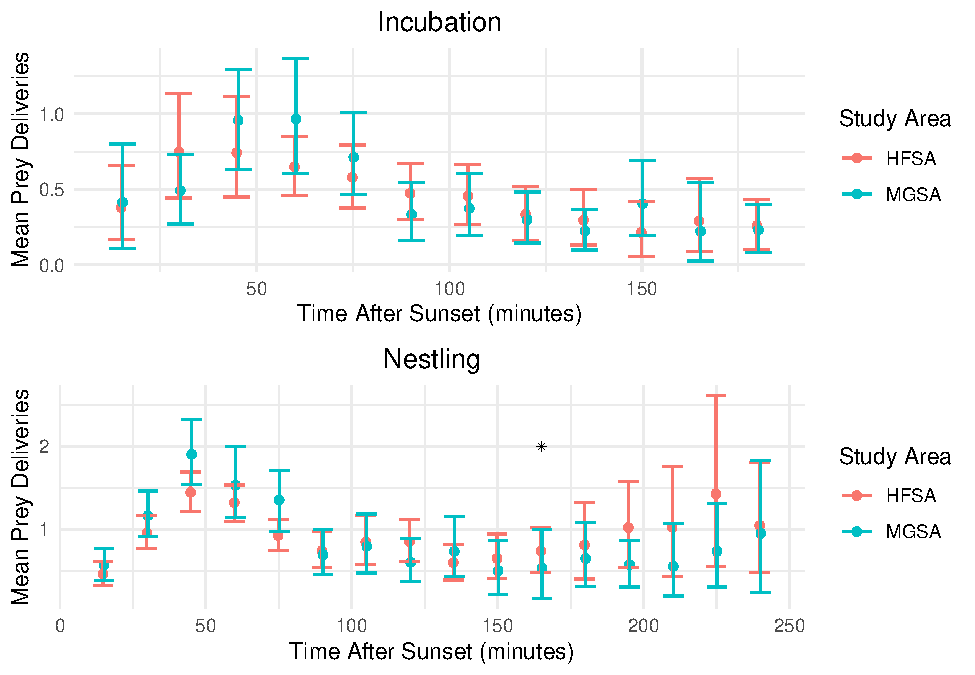
\includegraphics{../manuscript/figures/plot_site-1.pdf}
\caption{Mean prey deliveries during the incubation stage (top) and
nestling stage (bottom). Missouri Gulch Study Area (MGSA) is shown in
bue and Hayman Fire Study Area (HFSA) in red. Stars indicate significant
differences in medians based on unpaired two-sample Wilcoxon tests.}
\end{figure}

\hypertarget{discussion}{%
\section{Discussion}\label{discussion}}

Despite habitat devastation, Flammulated Owls continued to nest in the
Hayman Fire burn scar between 2004 and 2020 (Figure 1). Across study
sites, males were primarily responsible for nest provisioning, while
females were the sole incubators (Figure 2). Males delivered prey items
to females during the incubation period, with mean prey deliveries at
time = 235 and time = 250 showing no significant difference likely due
to a small sample size paired with high variation at these late hours of
the night. Once hatching occurred, females made some prey deliveries,
but the average rate of female prey deliveries was significantly lower
than that of male prey deliveries throughout the course of the night.

Almost no mean prey delivery rates were significantly different between
the HFSA and MGSA, with the exception of time = 165 during the nestling
stage (Figure 3). However, his does not appear to have biological
significance and would likely become insignificant with an increased
sample size.

This study has shown that across study site, males are the primary nest
provisioners, with females delivering small amounts of prey during the
nestling season. Decreased habitat quality in the Hayman Fire scar may
be putting more pressure on foraging males, who may have to travel
further to locate adequate foraging sites, thus increasing energy
demands. Although habitat quality continues to deteriorate, Flammulated
Owls still return to the HFSA each year to breed. The specialized
natural of their foraging habitat, combined with the males' inability to
adapt nest provisioning behavior following large-scale disturbance, may
be contributing to overall decreased annual survivorship for male
Flammulated Owls breeding in the Hayman Fire burn area.

\renewcommand\refname{References}
\bibliography{references.bib}

\end{document}
